
\subsection{Performance evaluation} 
\label{sec:CSORTBenchmarks}

\FloatBarrier

This section presents the experimental results. Our implementations of
counting sort are compared to the implementation of sorting from the
Thrust library \citecsort{THRUST}. Thrust is a C++ library, developed by
NVIDIA, which provides abstractions similar to the standard template
library, but targets the GPU. The reason we have chosen to compare with
Thrust is that it has similar goals to Obsidian: to provide high-level 
constructs while generating efficient GPU code.

All the data being sorted in the measurements are 32 bit unsigned
integer valued keys.
The convention used in the charts is that the y-axis represents time in ms. 
The different experiments are called {\em sorted} for sorting of an 
already sorted array, and {\em unique} for sorting of randomised arrays where each 
element occurs exactly once. There are also a number of experiments called 
T$x$ for a number $x$;  the arrays used in these experiments contain
elements from an interval of numbers (0 to $2^x-1$). 

Figures \ref{fig:chart1} and \ref{fig:chart3} show the results of
comparing our full counting sort to Thrust sort and occurrence sort
 to Thrust's {\tt sort} and {\tt unique} functions.
%% Figure \ref{fig:chart1}  show the results of
%% comparing our full counting sort to Thrust sort and our duplicate
%% removing sort to Thrust sort followed by unique.
Our implementation of
counting sort consistently outperforms Thrust, except for small ranges
of values. The reason counting sort performance degrades is that the
number of threads used in the reconstruct step is proportional to the
range, and therefore at small ranges the execution becomes more
sequential.

We compare occurrence sort to sort followed by unique from
the Thrust library because that seems to be the current best practice
\citecsort{REMOVEDUPS}. Our implementation is always at least twice as fast
but in many cases it outperforms Thrust by more than a factor of four.
Our method is clearly beneficial for removing duplicates.

%We are comparing 
%our implementations of counting sort to the sorting algorithm present 
%in the Thrust library. 
%The counting sort that removes duplicates is compared to Thrust's sort 
%followed by unique (unique removes all but one element in groups 
%of consecutively equal elements). These results can be found in 
%figures \ref{fig:chart1} and \ref{fig:chart3}. 

%We also compare our two variants of counting sort directly to each
We also compare occurrence sort and counting sort to each 
other.  The result of this is shown in figure \ref{fig:chart2}. We
can see that the occurrence sort is typically a factor of
two faster than the regular sorting algorithm. The speedup comes from
the fact that the {\tt occurs} kernel doesn't need to perform any kind
of synchronisation, whereas the {\tt histogram} kernel needs to use
atomic operations.

The charts included in this paper show the performance when sorting eight
respectively 32 million ($2^{23}$ resp. $2^{25}$) elements. However, we 
ran all benchmarks with a number of elements, $N$, equal to $2^{n}$ for $n$ 
between 20 and 25. We found that the interesting comparison is not in what 
happens as $N$ grows larger but rather what happens as we vary the ranges 
of the elements contained in the arrays. 
%% when the ranges of the 
%% elements contained in the array is increased. 

All timing was performed on a system with an NVIDIA GTX670 GPU.  
 
\begin{figure*}
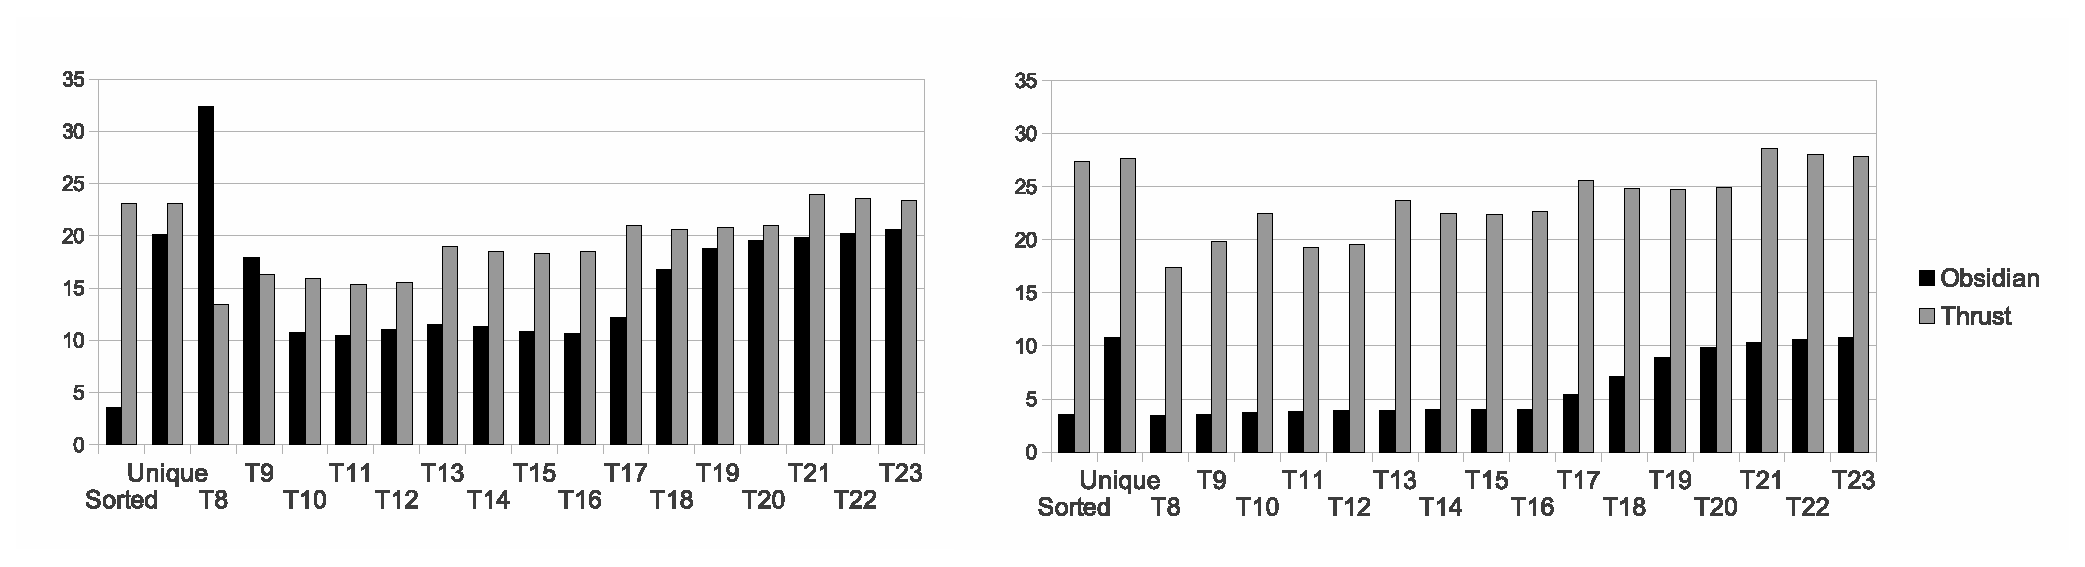
\includegraphics[width=\linewidth]{./csort/chart1}
\caption{On the left, counting sort is compared to the Thrust library. 
On the right, occurrence sort is compared to the {\tt sort} followed by {\tt unique} 
function in Thrust. Both charts show running time for 8 Million elements.}
%The left chart shows running time of full counting sort compared to 
%the sort function in the Thrust library. The right chart shows running time 
%of counting sort that removes duplicates compared to the sort followed by 
%unique function of the Thrust library. 8 Million elements where used in these 
%experiments.}
\label{fig:chart1}
\end{figure*}

\begin{figure*}
\includegraphics[width=\linewidth]{./csort/chart3}
\caption{This chart shows same comparison as figure \ref{fig:chart1}, but for 
32 Million elements.}
%The left chart shows running time of full counting sort compared to 
%the sort function in the Thrust library. The right chart shows running time 
%of counting sort that removes duplicates compared to the sort followed by 
%unique function of the Thrust library. 32 Million elements where used in 
%these experiments.}
\label{fig:chart3}
\end{figure*}


\begin{figure*}
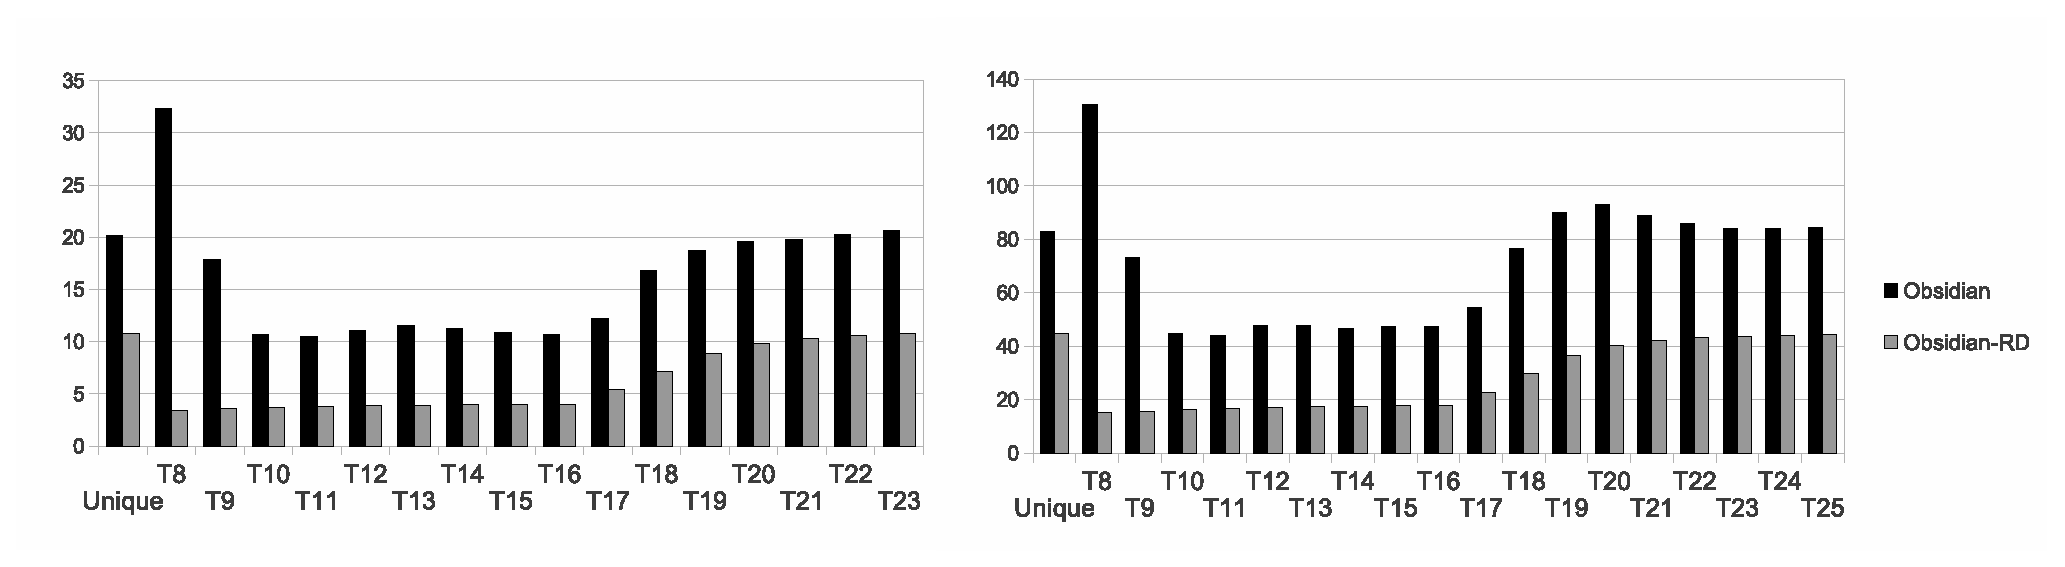
\includegraphics[width=\linewidth]{./csort/chart2}
\caption{These two charts compares occurrence sort to  counting sort. 
The left chart is for 8 Million elements and the right chart is 
for 32 Million elements.}
\label{fig:chart2}
\end{figure*}



\subsubsection{CUDA framework for the benchmarks}


To obtain the timing measurements above, a 
framework\footnote{Source code needed to repeat our experiments is available at \url{www.cse.chalmers.se/~joels/csort.html}} 
written in CUDA was used. 
This framework looks very similar to the CUDA code in figure \ref{fig:cudaCoord}. 
The main difference is that a number of kernels are run in sequence, as 
shown in figure \ref{fig:csortframe}. The timing is performed on the GPU 
computation only, as illustrated by figure \ref{fig:timing}.

\begin{figure} 
\begin{small}
\begin{verbatim} 
float total_time;

cudaEventRecord(start,0);
for (int i = 0; i < 1000; ++i) { 
    // perform counting sort. 
}
cudaEventRecord(stop,0);
cudaEventSynchronize(stop);
   
cudaEventElapsedTime(&total_time,start,stop);
\end{verbatim}
\end{small}
\caption{The timing methodology used in performance experiments. A CUDA event 
is recorded before and after the execution on the GPU. Their respective recorded times
are then compared.}
\label{fig:timing}
\end{figure}



\begin{figure} 
\begin{small}
\begin{verbatim} 
histogram<<<NB,BS,0>>>(dinput,dhistoutput);
  
scan256<<<NB,BS,2052>>>
    (dhistoutput,dscanoutput+1,dmaxs+1);
  
//dmaxs needs to be scaned (dmaxs2 is ignored) 
scan256<<<SMALL,BS,2052>>>
    (dmaxs+1,dmaxs+1,dmaxs1+1); 

scan16<<<1,SMALL,132>>>
    (dmaxs1+1,dmaxs1+1,dmaxs2); 

// distribute can be in-place regarding dresult 
// since it reads and writes in the exact 
// same location (per thread)
distribute<<<SMALL,BS,0>>>
    (BS,dmaxs1,dmaxs+1,dmaxs+1);
distribute<<<NB,BS,0>>>
    (BS,dmaxs,dscanoutput+1,dscanoutput+1);

reconstruct<<<NB,BS,0>>>
    (dscanoutput,dresult);   
\end{verbatim}
\end{small}
\caption{The kernel launch sequence used in the timing of counting sort for 
1 Million elements. Any other input data size would vary only some of the prefix 
sum (scan in the code) sizes.}
\label{fig:csortframe}
\end{figure}

% \FloatBarrier

%\begin{figure}
%\includegraphics[width=\linewidth]{./img/chartObs2M}
%\caption{Another chart example!}
%\label{fig:chart2}
%\end{figure}

%\begin{figure}
%\includegraphics[width=\linewidth]{./img/chartObs4M}
%\caption{Another chart example!}
%\label{fig:chart2}
%\end{figure}

%\begin{figure}
%\includegraphics[width=\linewidth]{./img/chartObs8M}
%\caption{Another chart example!}
%\label{fig:chart2}
%\end{figure}


%\begin{figure}[ht]
%\begin{minipage}[b]{0.5\linewidth}
%\centering
%\includegraphics[width=\textwidth]{./img/chartObs4M}
%\caption{This is to the left}
%\label{fig:figure1}
%\end{minipage}
%\hspace{0.5cm}
%\begin{minipage}[b]{0.5\linewidth}
%\centering
%\includegraphics[width=\textwidth]{./img/chartObs8M}
%\caption{This is to the right}
%\label{fig:figure2}
%\end{minipage}
%\end{figure}

%\begin{figure}
%\includegraphics[width=\linewidth]{./img/chart3}
%\caption{Shows execution of the counting sort algorithm on 4 million 
%         random elements.}
%\label{fig:chart3}
%\end{figure}

%Figures \ref{fig:chart1},\ref{fig:chart2} and \ref{fig:chart3} show how our algorithm 
%compares to a thrust implementation for 4,8 and 16 million elements in 
%various ranges.
 
% >>> What can be said more about the numbers ???
